\documentclass[12pt]{article}

\usepackage{float}
\usepackage{color}
\usepackage{caption}
\usepackage[margin=1in]{geometry}
\usepackage{amsmath}
\usepackage{xspace}
\usepackage{setspace}
\usepackage{lineno}
\usepackage{graphicx}
\usepackage{natbib}
\usepackage{subfigure}

\usepackage{multirow}

\begin{document}
\doublespacing
\linenumbers

\newcommand{\Lik}{\ensuremath{\mathcal{L}}\xspace}
\newcommand{\selac}{\emph{SelAC}\xspace}
\newcommand{\phydms}{\emph{phydms}\xspace}
\newcommand{\gy}{\emph{GY94}\xspace}
\newcommand{\ecoli}{\textit{E. coli}\xspace}
\newcommand{\PC}{physicochemical\xspace}

\newcommand{\beginsupplement}{%
  %%% commands for getting SM pages and figures labeled with S
  %% different than with other .cls
  \setcounter{section}{19} %appendix environment set in .cls file.  Set this to 19 to get an 'S' for figures
  \setcounter{page}{1}
  \renewcommand{\thepage}{S\arabic{page}} %this works

  \setcounter{table}{0}
  \renewcommand{\thetable}{S\arabic{table}}%
  \setcounter{figure}{0}
  \renewcommand{\thefigure}{S\arabic{figure}}%
}


\noindent RH: LANDERER ET AL.--- Estimating site specific selection
% put in your own RH (running head)
% for POVs the RH is always POINT OF VIEW
\bigskip
\medskip
\begin{center}

% Insert your title:
\noindent{\Large \bf Phylogenetic model of stabilizing selection is more informative about site specific selection than extrapolation from laboratory estimates.}
\bigskip

\noindent{C\textsc{EDRIC} ~{L\textsc{ANDERER}}$^{1,2,*}$,
B\textsc{RIAN} C.~ {O\textsc{MEARA}}$^{1,2}$,
\textsc{AND}
M\textsc{ICHAEL} A.~{G\textsc{ILCHRIST}}$^{1,2}$}

\end{center}

\vfill

{\small
\noindent$^{1}$Department of Ecology \& Evolutionary Biology, University of Tennessee, Knoxville, TN 37996-1610\\
\noindent$^{2}$National Institute for Mathematical and Biological Synthesis, Knoxville, TN 37996-3410\\
\noindent$^{*}$Corresponding author. E-mail:~cedric.landerer@gmail.com
}

\vfill
\centerline{Version dated: \today}
\vfill
\newpage

\begin{abstract}
Here we examine the adequacy of experimentally inferred site specific selection for amino acids to inform phylogenetic inferences of sequence evolution.
Previous work has shown that laboratory estimates of selection can improve model fit but did not assess their adequacy.

\end{abstract}
\newpage

\section*{Introduction}

Incorporation of selection into phylogenetic frameworks has already been a long lasting endeavor.
Early models focused the influence of selection on the substitution rate between a resident and a mutant \citep{GoldmanAndYang1994, MuseAndGaut1994, thorne1996}.
These models however, lack site specific equilibrium frequencies.
The importance of site specific equilibrium frequencies has long been noted \citep{felsenstein1981, gojobori1983}.
\citet{HalpernAndBruno1998} first introduced a framework to incorporate the site specific equilibrium frequencies of amino acids.
However, they had to concede that their model was to parameter rich and therefore intractable for biological data sets without simplifying assumptions.
More recent models that incorporate site specific equilibrium frequencies still require a large number of parameter to be estimated from the sequence data \citep{LartillotAndPhilippe2004,le2008,wang2008,holder2008,wu2013,tamuri2014}.
Other approaches treat site specific selection as a random effect \citep{rodrigue2010,rodrigue2013,rodrigue2014}.
A full parameterization requires $19\times L$ parameters were $L$ is the length of the sequence.
It therefore is an attractive option to utilize laboratory experiments to empirically estimate the site specific selection on amino acids \citep{bloom2014, thyagarajan2014, bloom2017}.

Deep mutation scanning (DMS) is often used to generate comprehensive fitness estimates of proteins \citep{Fowler2014}.
The quality of empirical estimates of site specific selection on amino acids from DMS depents on many factors, e.g. the initial library of mutants and the applied selection pressure.

Incorporating empirical estimates of site specific selection on amino acids has some important features.
Individual amino acid site along show differences in evolutionary rates strong preferences for amino acids \citep{HalpernAndBruno1998, ashenberg2013, echave2016}
The usage of site specific selection acknowledges the heterogeneity in selection along the protein sequence \citep{hilton2017}.
It reduces the number of parameters that have to be estimated from the data, making it applicable to smaller data sets and allowing for more complex models.
The incorporation of empirical estimates of selection does also have some shortcomings.
The need for empirical estimates of selection limits the application to fast growing organisms that can be manipulated under laboratory conditions.
This limits the application of experimentally informed models as many organims can not be cultivated under laboratory conditions or have a to long generation time.

Even in the cases were empirical estimates of site specific selection on amino acids can be optained their usefulness for phylogenetic reconstruction is not yet fullly clear.
In this study, we assess the adequacy of experimentally inferred site specific selection using DMS to inform phylogenetic models.
We use site specific estimates of slection on amino acids for the $\beta$-lactamase TEM from \citet{stiffler2016}.
We find that experimentally inferred selection does not adequatly reflect evolution in the wild.
In contrast, \selac a mechanistical phylogenetic model of stabilizing selection rooted in first princibles with site specific equilibrium frequencies improves model fit, and better reflects evolution in the wild \citep{beaulieu2018}.
\selac does not require extensive laboratory estimates for site specific selection on amino acids.
\selac assumes that the distance of two amino acids in \PC space affects substitution probabilities and estimates only one discrete parameter per site, the optimal amino acid at a site.
Therefore \selac only requires $19$ site specific parameters instead of $19\times L$.

\section*{Results}
\subsection*{Site Specific Stabilizing Selection on Amino Acids Improves Model Fit}
We compared the models \phydms \citep{hilton2017} and \selac, models of stabilizing site specific amino acid selection, to 281 other codon and nucleotide models by fitting them to 49 sequences of the $\beta$-lactamase TEM.
Models with site specific selection on amino acids improved model fits by 917 to 1483 AICc units over codon or nucleotide models without site specific selection (Table \ref{tab:AIC}).
In addition, \selac does outperform \phydms by 560 to  566 AICc units.

\selac utilizes a hierarchical model framework and estimates 263 site specific parameters, $\sim5\%$ of the 4997 parameters necessary to fully describe the site specific selection on amino acids.
In contrast, \phydms does not infer any site specific parameters, but utilizes site specific selection on amino acids estimated from deep mutation scanning experiments.
Incorporating site specific selection on amino acids estimated from deep mutation scanning experiments into \selac (\selac+DMS) yields a similar AICc value to \selac without that information.
However, \selac+DMS is favored by AICc.
This is solely due to a decrease in the number of parameters estimated, as the $\log(\Lik)$ decreases from $-1498$ to $-1768$ (Table \ref{tab:AIC}).
The number of parameter for \selac, however, is reported conservatively as the number of unique site patterns in the TEM alignemnt is only 27 and thus the number of paramters would be 123.
This however is likely an under estimate of the degrees of freedom and the true number of parameters remains unclear at this point.

\begin{table}
  \centering
  \begin{tabular}{lrrrrrr}
    Model		& $\log(\Lik)$ &$n$ & AIC & $\Delta$AIC & AICc & $\Delta$AICc\\ \hline 
    \selac		& -1498 & 374& 3744&  0 	& 3766  & 6 \\
    \selac+DMS 		& -1768 & 111& 3758& 14	& 3760  & 0\\
    \phydms 		& -2061 & 102& 4326& 582& 4328 & 568\\
    SYM+R2 		& -2230 & 102& 4663& 919& 4694 & 934 \\
    GY+F1X4+R2 		& -2243 & 102& 4690& 946& 4821 & 1061 \\
  \end{tabular}
  \caption{Model selection, shown are the three models of stabilizing site specific amino acid selection (\selac, \selac+DMS, \phydms) and the best performing codon and nucleotide model. See full table for all 231 models}
  \label{tab:AIC}
\end{table}

Interestingely, the best codon model (\gy) \citep{GoldmanAndYang1994} is outperformed by a variety of nucleotide model e.g. \emph{SYM} \citep{zharkikh1994}.
This indicates that negative frequency dependent selection like it is modeled in \gy is not appropriate for TEM \citep{beaulieu2018}.
Figure \ref{fig:phylo} shows that the estimated phylogenetic trees shift from long terminal branches (\selac) to longer internal branches (\phydms, \gy).
All models produce polytomies but their location differs along the phylogeny between models.
The largest polytomies appear in the experimentally informed phylogenies.

\begin{figure}[H]
     \centering
	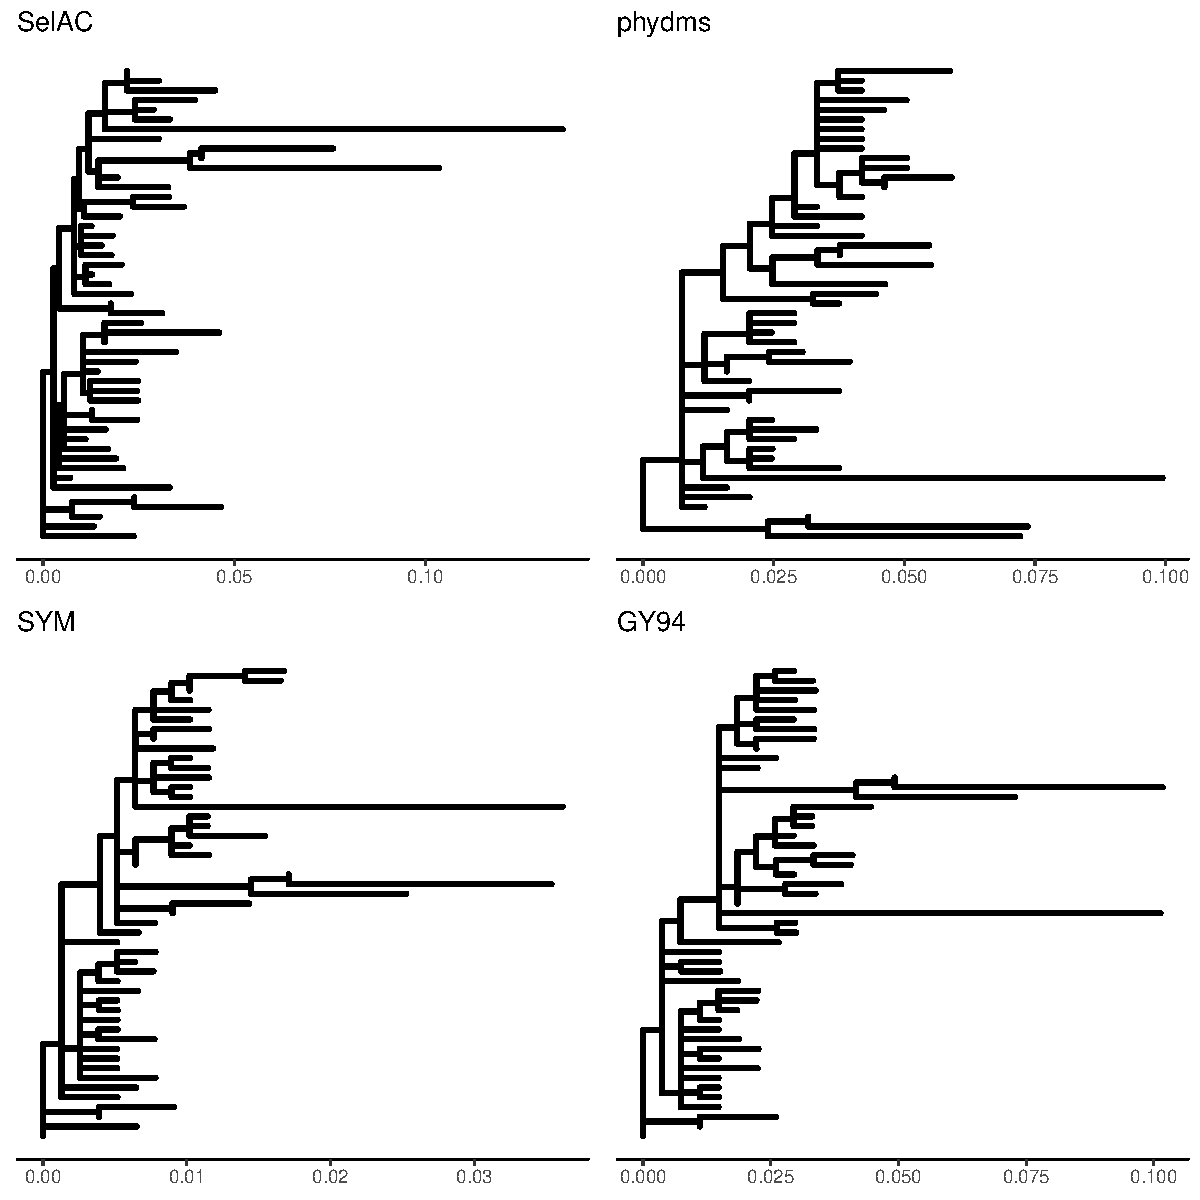
\includegraphics[width=\textwidth]{img/phy_TEM2016.pdf}
	\caption{Phylogenies estimated using \selac, \selac+DMS, \phydms, and \gy.}
	\label{fig:phylo}
\end{figure}

\subsection*{Laboratory Inferences of Selection are inconsistent with Observed Sequences.}
Improved model fits with phydms are deceiving.
The site specific selection inferred by the deep mutation scanning experiment is inconsistent with the observed TEM sequences.
We find that the sequence of selectively favored amino acids has only $52 \%$ sequence similarity with the observed consensus sequence (Figure \ref{fig:sim_seqs_cons}).
This is in contrast to the 99 \% of sequence similarity with the sequence of selectively favored amino acids estimated by \selac.

\begin{figure}[H]
     \centering
	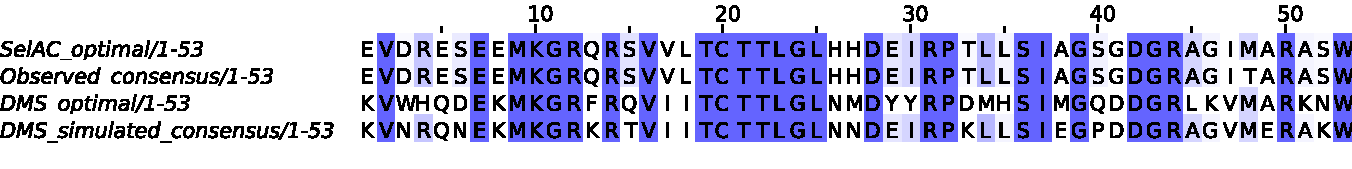
\includegraphics[width=\textwidth]{img/seq_simil_short.pdf}
	\caption{Every 5th residue. DMS and simulation based on DMS do not reflect natural sequences}
	\label{fig:sim_seqs_cons}
\end{figure}

Simulations of codon sequences under the experimentally inferred site specific selection for amino acids reveals that we would not expect to see the observed TEM sequences.
We simulated under a wide range of effective population sizes $N_e$, and find that the experimentally inferred site specific selection is very strong.
Only when $N_e$ is on the order of $10^0$ drift is overpowering the efficacy of selection.
With realistic values for $N_e = 10^7$, we find that the simulated sequences to show sequence similarity of $62 \%$ with the observed consensus sequence (Figure \ref{fig:dms_sim}a).
This is a higher similarity than the observed consensus sequence shows with the the sequence of selectively favored amino acids estimated using deep mutation scanning.
The genetic load of the simulated sequences deacrease slowely with increasing $N_e$ (Figure \ref{fig:dms_sim}b).
At time 1 and $N_e = 10^7$ the simulated sequences show a genetic load of 0.25, which is in contrast to the $\sim 8$ times higher observed load of 2.1.
Thus it appears unlikely that the observed sequences have evolved under the experimentally inferred site specific selection for amino acids.


\begin{figure}[h]
    \centering
    \begin{subfigure}
        \centering
        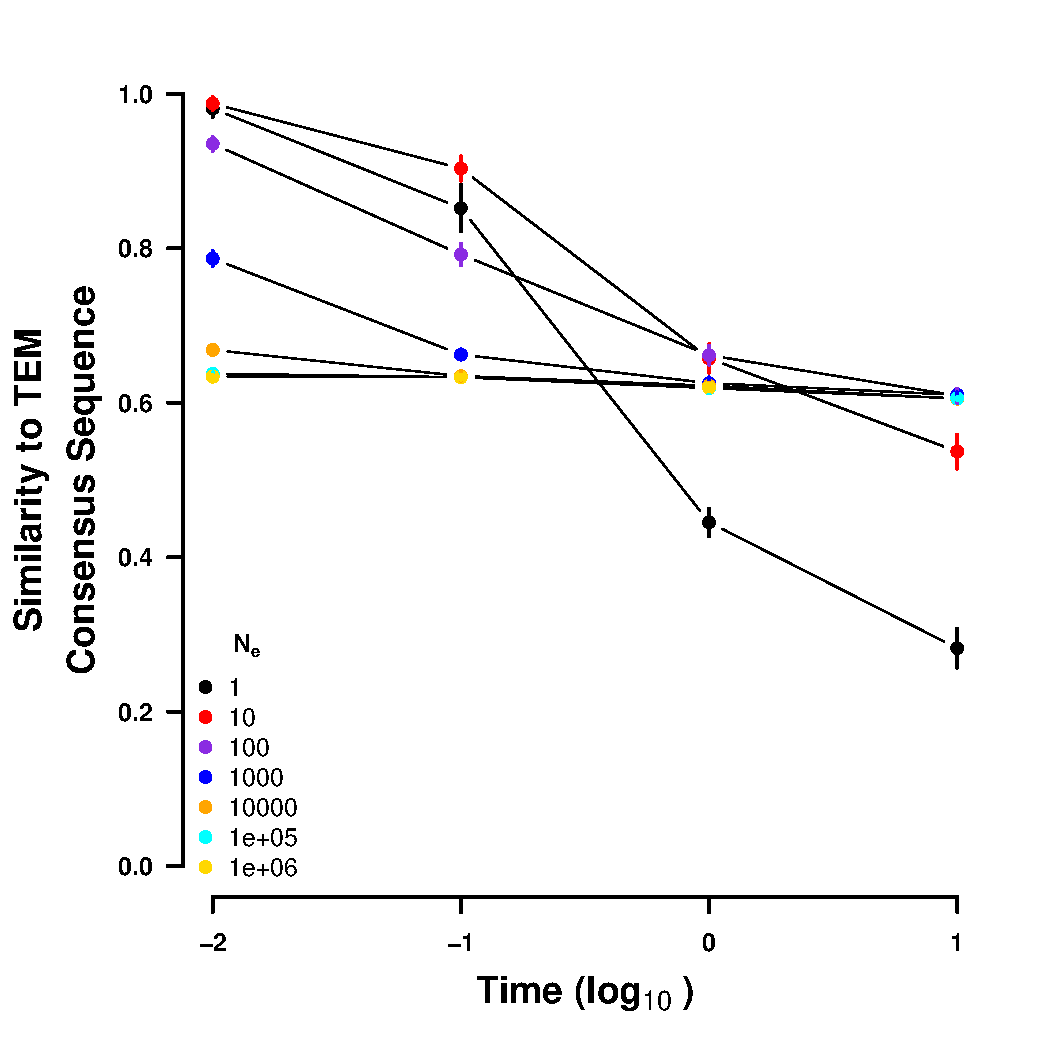
\includegraphics[width=.45\textwidth]{img/simulated_dist_time_DMS_ancest.pdf}
    \end{subfigure}
    \begin{subfigure}
        \centering
        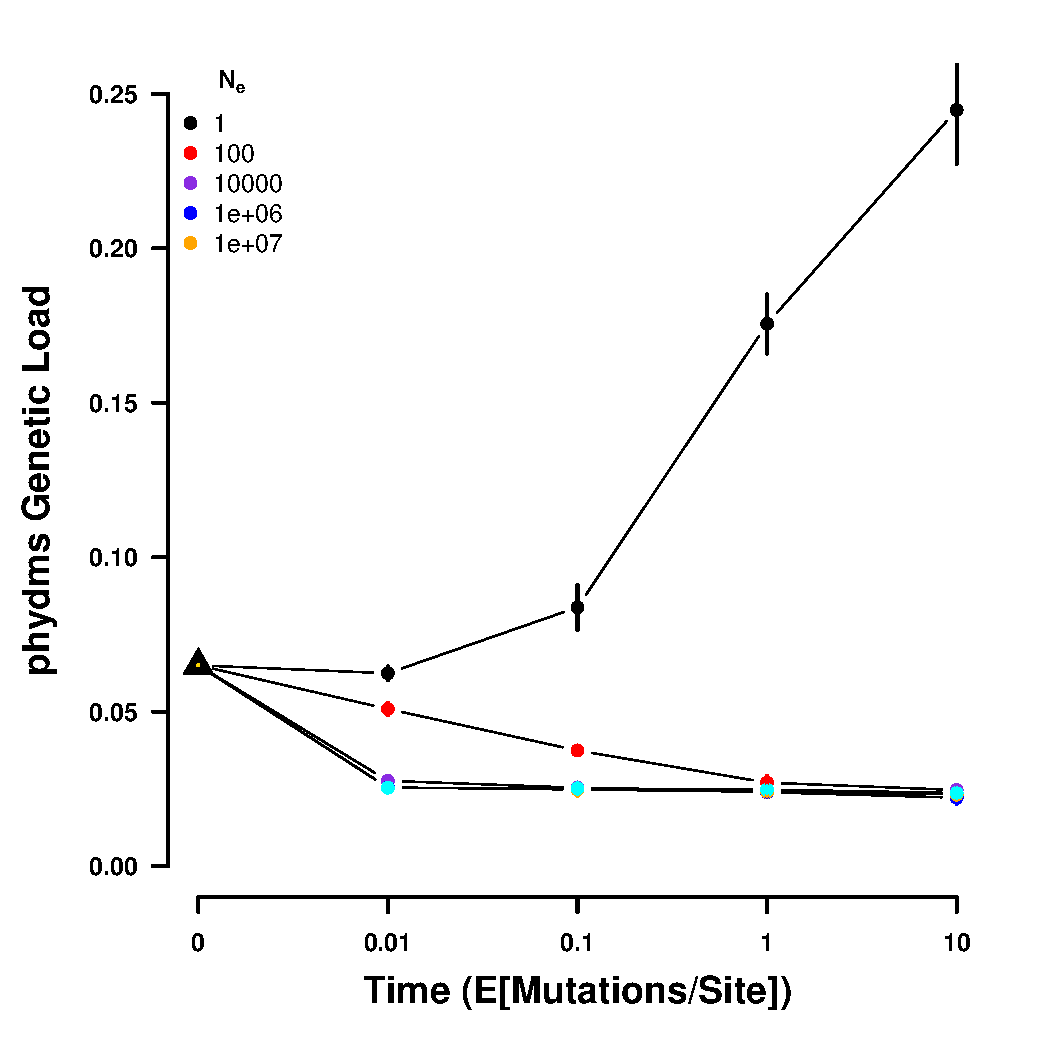
\includegraphics[width=.45\textwidth]{img/simulated_gl_time_DMS_ancest.pdf}
    \end{subfigure}
    \caption{Sequences simulated from the ancestral state under the site specific selection on amino acids estimated using deep mutation scanning. 
    (left) Sequence similarity to the observed consensus sequence at various times for a range on values of $N_e$.
    (right) Genetic load of the simulated sequences at various times for a range on values of $N_e$.
    Time is given in number of expected mutations.
    Points indicate sample means and vertical bars indicate standard deviations. Initial sequence is the inferred ancestral state of the TEM variants and not shown.}
    \label{fig:dms_sim}
\end{figure}

\subsection*{Stabilizing Selection for Optimal Physicochemical Probabilities increases Model Adequacy} 
We assessed model adequacy and find that \selac better explains the observed TEM sequences.
The observed consensus sequence has a very high sequence similarity with the sequence of selectively favored amino acids estimated by \selac (99 \%).
Furthermore, assuming the site specific selection estimated by \selac, the observed sequences only show a minimal genetic load (Table \ref{tab:selection}, Figure \ref{fig:tem2016_sse}).

We simulated codon sequences forward in time for various length of time to assess the sequence similarity, assuming the \selac inferred site specific selection for amino acids.
% Ancestral starting point
We simulated the evolution of TEM from the inferred ancestral state using a wide range of effective population sizes $N_e$ (Figure \ref{fig:selac_sim}a).
The ancestral state state was estimated to be the observed consensus sequence.
For small $N_e$, we find that sequences drift away from the observed consensus. 
In turn, the genetic load increases drastically.
With increasing $N_e = 10^7$ the simulated sequences reach a sequence similarity at time 1 of $83 \%$, this is in contrast to the observed sequence similarity $98 \%$.
We calculated the genetic load at this time of the simulated sequences to be $9.8\times10^{-6}$ (Figure \ref{fig:selac_sim}b).
The genetic load of the observed sequences is estimated $4.2\times 10^{-5}$, one order of magnitute higher.
Thus, the simulated sequences show a lower genetic load despite the greater divergence from the observed consensus sequence.


\begin{figure}[h]
    \centering
    \begin{subfigure}
        \centering
        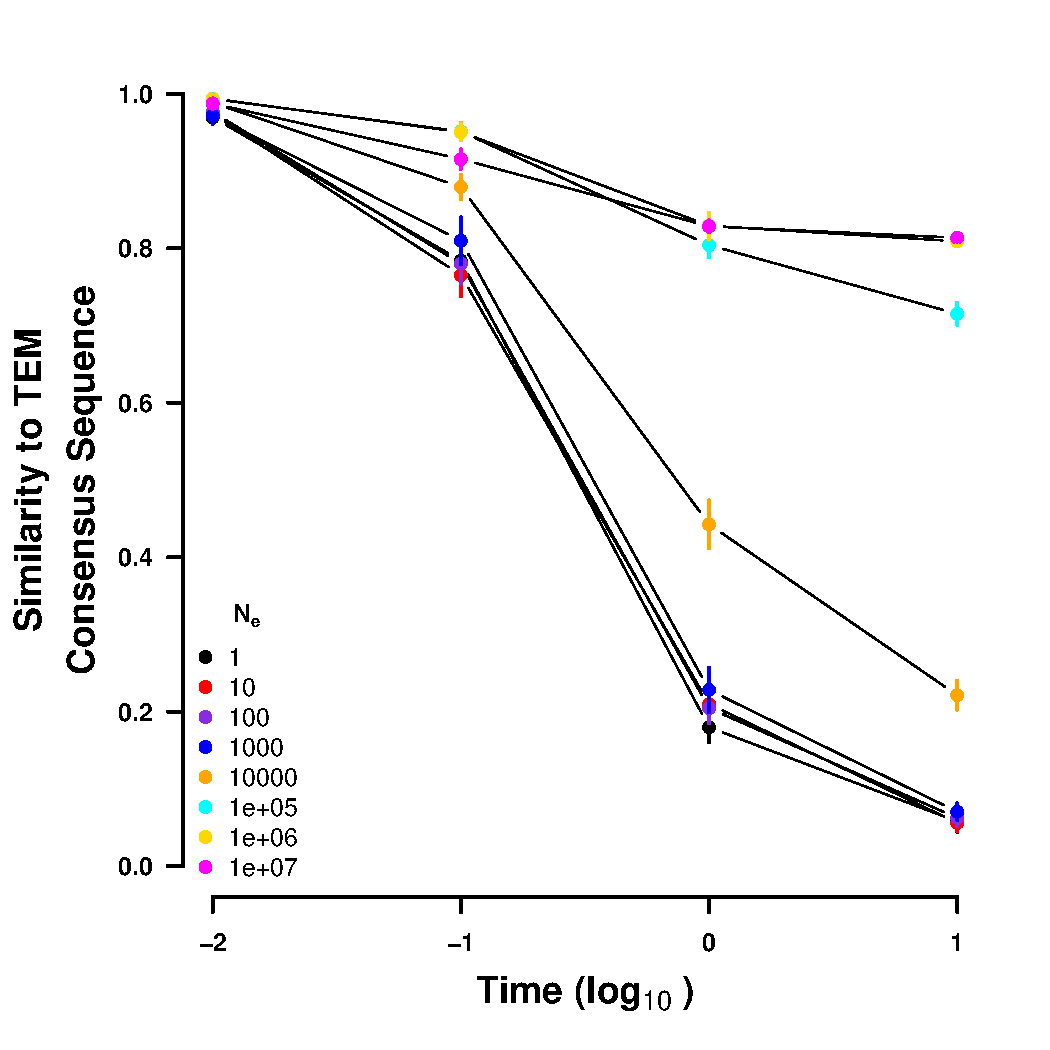
\includegraphics[width=.45\textwidth]{img/simulated_dist_time_SELAC_ancest.pdf}
    \end{subfigure}
    \begin{subfigure}
        \centering
        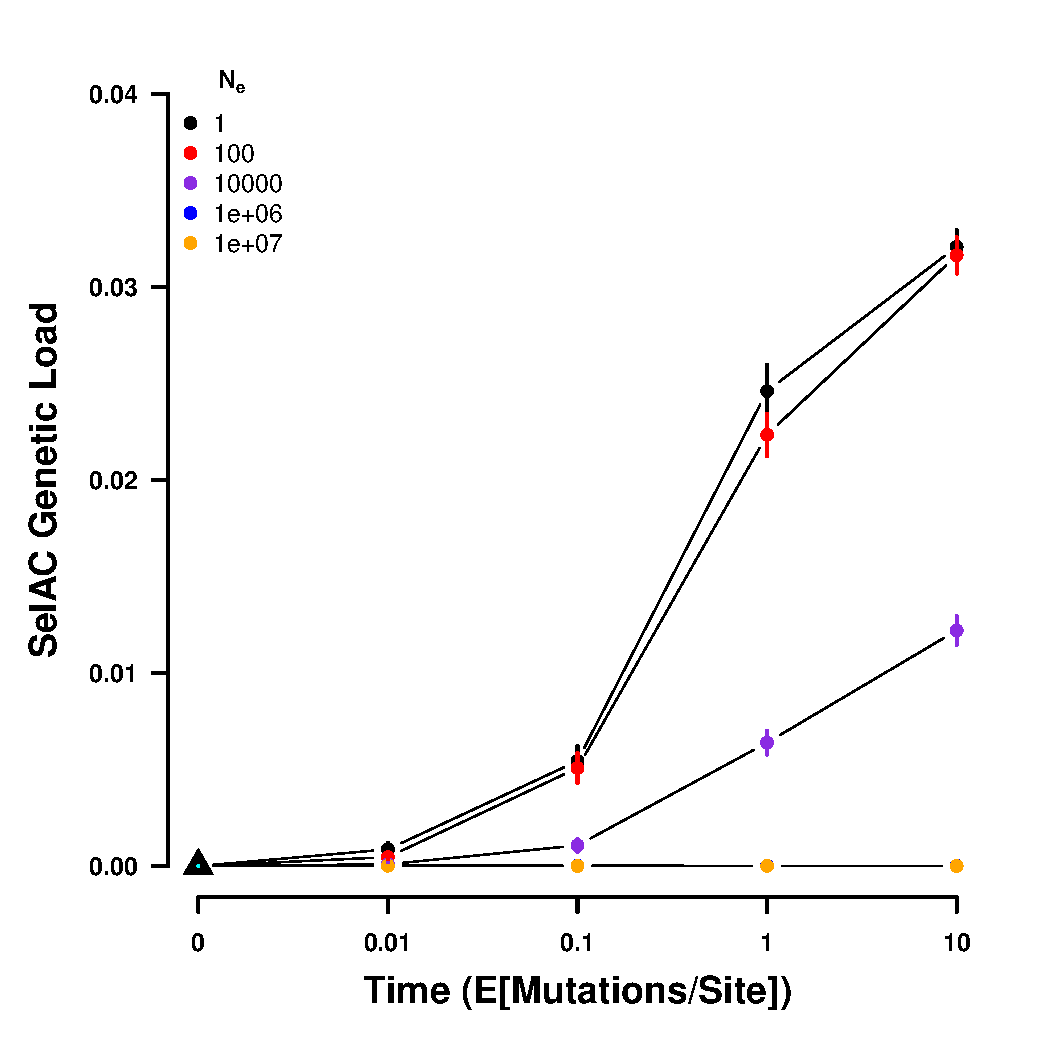
\includegraphics[width=.45\textwidth]{img/simulated_gl_time_SELAC_ancest.pdf}
    \end{subfigure}
    \caption{Sequences simulated from the ancestral state under the site specific selection on amino acids estimated using \selac. 
    (left) Sequence similarity to the observed consensus sequence at various times for a range on values of $N_e$.
    (right) Genetic load of the simulated sequences at various times for a range on values of $N_e$.
    Time is given in number of expected mutations.
    Points indicate sample means and vertical bars indicate standard deviations. Initial sequence is the inferred ancestral state of the TEM variants and not shown.}
    \label{fig:selac_sim}
\end{figure}

% Random starting point
To further demonstrate the consistency of \selac, we utilized random codon sequences as starting points.
We find that the sequence similarity increases with effective population size $N_e$.
The random sequences start of with a similarity of $\sim6 \%$ which increases with $N_e$ to $\sim28 \%$ (Figure \ref{fig:selac_sim_rand}a).
The same initial sequences under the site specific selection inferred by the deep mutation scanning experiment increase only to $\sim18 \%$ in sequence similarity.



\subsection*{Site Specific estimates of Selection on Amino Acids}
\selac allows for the site specific estimation of selection on amino acids and the genetic load of an observed amino acid relative to the inferred optimal amino acid.
We find that the genetic load is distributed along most of the observed TEM sequence with the exception of the region between residue 80 to 120 were three consequtive helices are located (Figure \ref{fig:tem2016_sse}). 
The most noticable increases in genetic load are found in unstructured regions
The largest increase in genetic load however, is located at the begining of the last helix.
We therefore estimate similar genetic loads for helices and unstructured regions in the observed TEM sequences (Table \ref{tab:selection})
The highest 
The Active sites appear to be under the strongest selection, with no accumulated genetic load.
This is in concordance with the experimental estimates.

\begin{table}
  \centering
  \begin{tabular}{llrrrr}
    & & \multicolumn{2}{c}{G} & \multicolumn{2}{c}{Genetic Load} \\ 
    Protein & Secondary Structure	& \multicolumn{1}{c}{Mean} & \multicolumn{1}{c}{SE} & \multicolumn{1}{c}{Mean} & \multicolumn{1}{c}{SE} \\ \hline 
    TEM	&		& 219.3 & 7.5 & $0.16\times10^{-7}$ & $6.5\times10^{-8}$ \\
    &Helix 		& 206.1 & 12.4 & $0.18\times10^{-7}$ & $0.13\times10^{-7}$ \\
    &Beta Sheet 	& 238.6 & 15.8 & $6.8\times10^{-8}$ & $2.9\times10^{-8}$ \\
    &Unstructured 	& 224.8 & 11.4 & $0.19\times10^{-7}$ & $8.1\times10^{-8}$ \\
    &Active Sites 	& 300   & 0    & 0      & 0      \\ \hline
    
    SHV&		& 244.9 & 6.8  & $4.0\times10^{-8}$ & $1.9\times10^{-8}$ \\
    &Helix		& 234.6 & 11.5 & $7.3\times10^{-8}$ & $4.8\times10^{-8}$ \\
    &Beta Sheet 	& 253.1 & 12.8 & $2.1\times10^{-8}$ & $1.1\times10^{-8}$ \\
    &Unstructured	& 250.3 & 11.0 & $1.8\times10^{-8}$ & $59\times10^{-8}$  \\
    &Active Sites	& 199.9 & 100  & $2.4\times10^{-8}$ & $2.4\times10^{-8}$ \\

  \end{tabular}
  \caption{Efficacy of selection (G) and Genetic Load for TEM and SHV and separated by secondary structure. UPDATE TABLE, MAKE EVERYTHING 10-8}
  \label{tab:selection}
\end{table}

It was previously proposed that experimentally inferred site specific selection for amino acids can be used to extraplotate the fitness landscape of related proteins \citep{bloom2014}.
We therefore compared the site specific efficacy of selection G, the \selac selection parameters of our \selac TEM model fit to a \selac model fit of SHV, and genetic load.
We find that site specific efficacy of selection G differes greatly between SHV and TEM ($\rho = 0.12$), despite a similar estimate of the parameter $\alpha_G$ describing the distribution of G values (Figure \ref{fig:tem_shv_param_comp}a).
With the expection of the active site, we find that G is increased in SHV (Table \ref{tab:selection}).
In general, most \selac selection parameters are very similar between the TEM and the SHV model fit. 
An exception is the weight for the \PC composition property $\alpha_c$ (Figure \ref{fig:tem_shv_param_comp}b).

\begin{figure}[H]
     \centering
	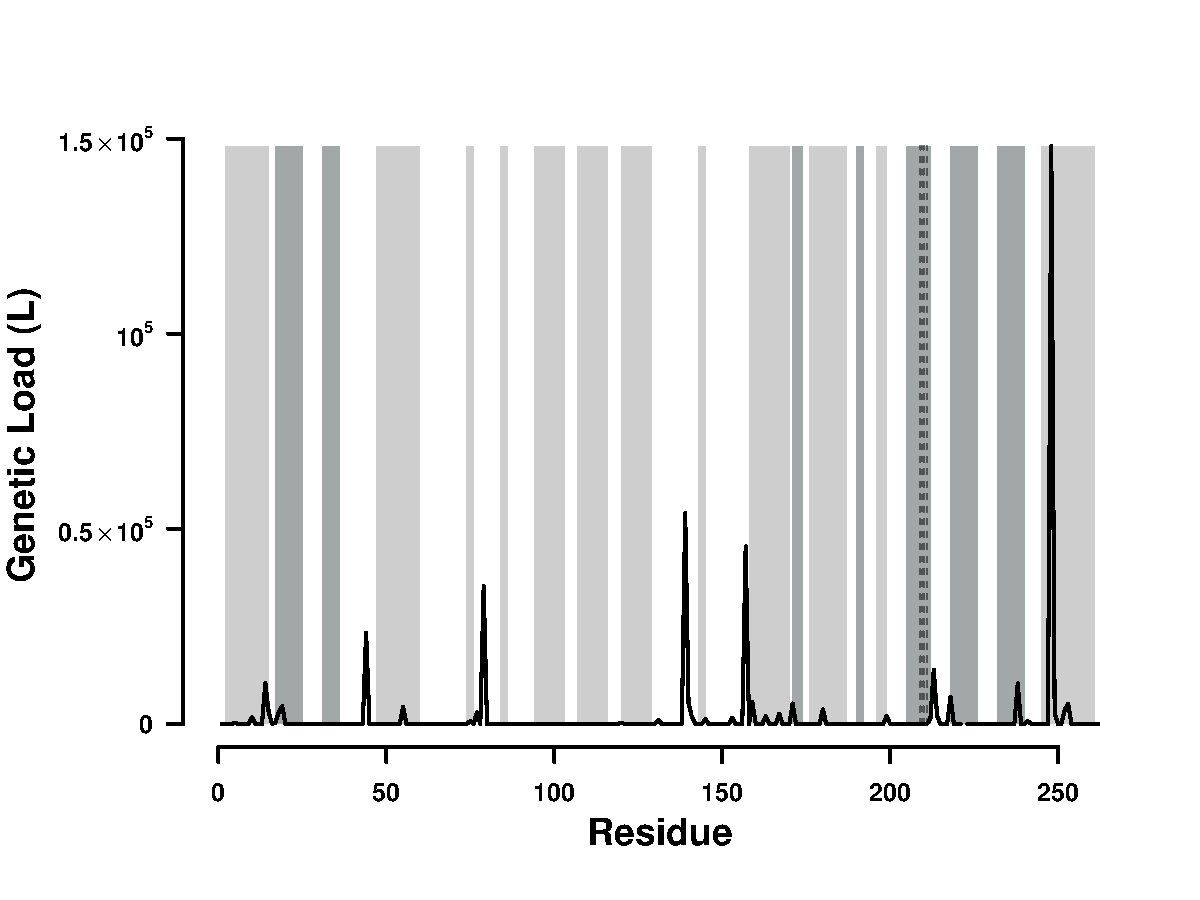
\includegraphics[width=\textwidth]{img/GL_slide_TEM2016}
	\caption{TEM, bars are different secondary structure elements. Dashed dotted line is DMS, solid is SelAC sNe, all lines are means of all sequences. vertical lines are active/binding sites.}
	\label{fig:tem2016_sse}
\end{figure}

The genetic load in SHV is by an order of magnitute lower than in TEM with the exception of residues found in $\beta$-sheets and the active site (Table \ref{tab:selection}).
This is consitent with the elevated site specific efficacy of selection G in SHV.
As a comparison of site specific efficacy of selection G already indicated, the sites introducing genetic load differ between SHV and TEM (Figure \ref{fig:shv2016_sse}).
We find the highest genetic load in SHV at the end of the first helix.
However, we do find a peak of similar magnitute in the TEM sequence at the end of the first helix.


\section*{Discussion}

Here we revisited how well experimental selection estimates from laboratory experiments, specifically deep mutation scanning, explain sequence evolution and compared it to \selac, a novel phylogenetic framework.
Previous work has shown that laboratory estimates of selection can improve model fit over classical approaches like GY94 \citep{bloom2014, bloom2017}.
While our study confirms this notion, we identify improtant shortcomings of these laboratory estimates.
In contrast, \selac is a more general phylogenetic model of stabilizing selection that does not depend on costly laboratory estimates of selection and is favored by model selection (Table \ref{tab:AIC}).

While previous work showed the advantages of experimentally informed phylogenetics estimates, they did not assess how adequate the estimated selection reflects observed sequences.
This becomes abherent in the low sequence similarity between the observed consensus sequence and the sequence of selectively favored amino acids estimated from deep mutation scanning experiments.
This begs the question how well the experimental selection coefficients represent evolution in the wild.
Deep mutation scanning experiments are performed using a comprehensive library of mutants and a strong artificial selection pressure \citep{FirnbergAndOstermeier2012, Jain2014, FowlerAndFields2014, Fowler2014}.
This results in a very large selection coefficient $s$ and a competing heterogeneous population.

The induced selection pressure during the deep mutation scanning experiment was limited to ampicillin \citep{stiffler2016} and focused on the TEM-1 variant.
However, TEM can also confer resistance to a wide range of other antibiotics, like other penicillins, cephalosporins, cefotaxime, ceftazidime, or aztreonam \citep{sougakoff1988,sougakoff1989,goussard1991,mabilat1992,chanal1992,brun1994}.
Thus, the inferred selection is biased towards ampicillin and as our simulations show does not reflect the evolution the observed TEM variants have experienced (Figure \ref{fig:dms_sim}).
This may very well be very appropriate to explore the selection on TEM in a modern hospital environment but is unlikely to be applicable to the selection faced in the wild.
We therfore propose to include a variety of selection pressures if the experimental selection estimates are used for phylogenetic inference.

%TODO:  Lack of repeatability between labs introduces further problems (Firnberg et al 2014 vs. Stifler et al. 2016).

If we assume that the experimental selection estimates underly the evolution of the observed TEM sequences we are left with two possible explanations for the observed sequences.
First, the sequences are unable to reach a fitness peak, potntially due to a lack of selection of not enough time.
Second, the observed TEM sequences are mal-adapted.
Both options seem unlikely.
\ecoli has a large effective population size $N_e$, estimates are on the order of $10^8$ to $10^9$ \citep{OchmanAndWilson1987, hartl1994}.
As new mutations are introduced into a population proportional to $N_e$, \ecoli can effectively explore the sequence space.
We therefore expect the observed sequence variants to be near mutation-selection-drift equilibrium.
This is confirmed by our simulations as we would expect to observe a higher sequence similarity and decreased genetic load even with much smaller $N_e$ (Figure \ref{fig:dms_sim}).
Previous work showed that TEM the catalytic reaction of penicillin-class antibiotics is close the diffusion limit, making TEM a so-called perfect enzyme \citep{matagne1998}.

As experimental selection estimates are not readily available, one solution is to extrapolate the estimates to homologeous gene families \citep{bloom2014, bloom2017}.
When extrapolating the selection estimates from the $\beta$-lactamase family TEM to SHV, the sequence similarity between the observed consensus sequence and the sequence of selectively favored amino acids estimated from deep mutation scanning experiments drops rom $52 \% $ to $49 \%$.
Comparrison of the site specific efficacy of selection (G) revealed large differences in the site specific selection on amino acids between TEM and SHV.
The missmatched in \PC weights also indicates differences in selection constrains. 
While the polarity of amino aicds is of similar importance in TEM and SHV, amino acid composition plays a much greater role in SHV than in TEM.

In contrast to the experimental selection estimates, the \selac selection estimates are consistent with the observed sequences, e.g. the selectively favored amino acids estimated by \selac shows a high sequence similarity with the observed consensus sequence ($99 \%$).
\selac does not rely on artifically induced selection in the laboratory but is a mechanistical framework rooted in first princibles.
It estimates site specific selection on amino acids from the seqeuence data based on distances between amino acids in \PC space \citep{grantham1974,beaulieu2018}.
This allows \selac to be applied to any set of protein coding sequences, eliminating the need to extrapolate from one homologeous gene family to the next (e.g. from TEM to SHV).

While \selac better explains the observed TEM sequences than the experimental estimates of site specific selection on amino acids, it is not without shortcomings itself.
While \selac allows for site heterogeneity in selection for amino acids, it still assumes multiplicative fitness across all sites and therfore ignores epistatis.
This however, is a shortcoming shared with experimental estimates by deep mutation scanning, as each mutation typically only carries one mutation \citep{FirnbergAndOstermeier2012, Jain2014}.
\selac is a model stabilizing selection, however, not every protein is under stabilizing selection.
TEM playes a role in chemical warfare with conspecifics and other microbes, therfore some sites may be under negative frequency dependent selection.
This potential heterogeneity in selection highlights another shortcoming of \selac.
\selac assumes the same distribution for the efficacy of selection (G) across the whole proteins.
However, it is easy to imagine that sites in different secondary structures or at active sites do not share a common distribution.

As \selac assumes that the fitness of an amino acid at a site declines with its distance in \PC space to the optimal amino acid, the choice of \PC properties becomes important.
In this study, we assumed the \PC properties estimated by \citet{grantham1974} for all sites.
However, a wide range of \PC properties of amino acids have been assessed.
A more optimal choice of \PC properties may be possible as well as the a relaxation of the assumptions that the same properties apply to all sites equally.
The hierarchical model structure allows to easilly address these shortcoming as needed.

In conclusion, experimental estimates of site specific selection on amino acids have to be treated with great care and their adequacy should be assessed before informing phylogenetic studies.
We also show that information on site specific selection on amino acids can be extracted from sequence data with mechanistical models rooted in first princibles.

\section*{Materials and Methods}

\subsection*{Phylogenetic Inference and Model selection}

TEM and SHV sequences were obtained from \citet{bloom2017} already aligned.
We however, separated the TEM and SHV sequences into individual alignemnts.
Experimentally fitness values for TEM were taken from \citet{stiffler2016}.
We followed \citep{bloom2017} to convert the experimental fitness values into site specific equilibrium frequencies for \phydms. 

\selac (version 1.6.1) was fitted to the TEM alignment using R (version 3.4.1) \citep{rcore} with and without site specific selection on amino acids estimated from deep mutation scanning experiments.
We assumed the \PC properties estimated by \citet{grantham1974}.
\phydms (version 2.5.1) was fitted using site specific selection on amino acids estimated from deep mutation scanning experiments from \citet{stiffler2016} and python (version 3.6).
All other models were fitted using IQTree \citep{nguyen2015}.

We report each model's $\log(\Lik)$, AIC, and  AICc. 
Models were selected based on the AICc values.

\subsection*{Sequence Simulation}

Sequences were simulated by stochastic simulations using a Gillespie algorithm \citep{gillespie1976} that was model independent.
The simulation followed \citet{SellaAndHirsh2005} to calculate fixation probabilities.
The fitness values were estimated using \selac or experimentally inferred.
We chose the fitnest values of the highest concentration (2500 $\mu g/mL$) treatment of ampicillin for our comparison.
We modified the experimental fitness such that the amino acid with the highest fitness at each site has a value of one.
Mutation rates were taken from the \selac or \selac+DMS fit.
The initial sequences were either a random sample of 263 codons or the ancestral sequence reconstructed using FastML \citep{fastml} (last accessed: 30.09.2018).
Each sequence was simulated 10 times and we report average genetic load and sequence similarity and the corresponding standard error.
The sequences were sampled at times 0.01, 0.1, 1, and 10 expected mutations per site.

\subsection*{Estimating site specific G}



\subsection*{Estimating site specific fitness values $w_i$}

Following \citet{beaulieu2018} $w_i$ is proportional to
\begin{equation}
w_i \propto \exp(-A_0\eta\psi)
\end{equation}
were $A_0$ decribes the decline in fitness with each high energy phosphate bond wasted per unit time, and $\psi$ is the protein's production rate.
$\eta$ is the cost/benefit ratio of a protein (see \citep{beaulieu2018} for details). 
However, \selac only estimates a composition parameter $\psi' = A_0\psi N_e$.
$N_e$ describes the effective population size.
\selac assumes $N_e = 5\times 10^6$.
\selac assumes $A_0 = 4 \times 10{-7}$ \citep{gilchrist2007}.
Thus, 
\begin{equation}
\psi = \frac{\psi'}{A_0N_eq}
\end{equation}


\subsection*{Model Adequacy}

Model adequacy was assessed by comparing the observed sequences and simulations under the site specific selection inferred by the deep mutation scanning experiment or \selac.
First, similarity between the sequence of selectively favored amino acids and the observed TEM sequences was assessed.
Sequence similarity was measured as the number of differences in the amino acid sequence.
Second, the genetic load of the observed and the simulated sequences was calculated using either the site specific selection inferred by the deep mutation scanning experiment or \selac.

Genetic load was calculated as
\begin{equation}
L_i = \frac{w_{max} - w_i}{w_{max}}
\end{equation}
were $w_{max}$ is the fitness of the sequence of selectively favored amino acids estimated using  the site specific selection inferred by the deep mutation scanning experiment or \selac.
$w_i$ represents the fitness of the $i$th residue.
This the genetic load $L$ of a sequence is given by $\sum_{i=1}^n L_i$ where $n$ is the number of amino acids.



\bibliographystyle{unsrtnat}
\bibliography{ecoli}

\clearpage
\beginsupplement
\section*{Supplementary Material}


\begin{figure}[H]
     \centering
	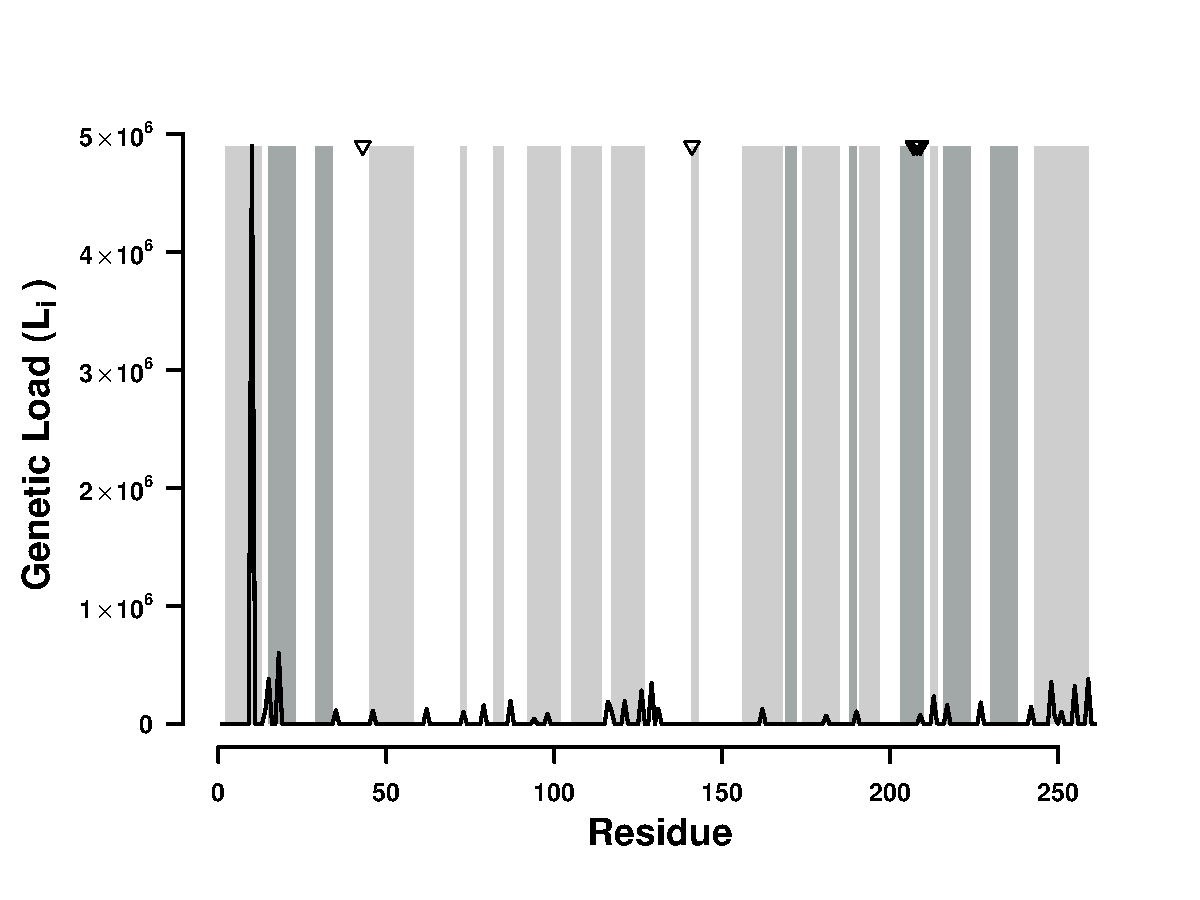
\includegraphics[width=\textwidth]{img/GL_slide_SHV2016}
	\caption{SHV, bars are different secondary structure elements. Dashed dotted line is DMS, solid is SelAC sNe, all lines are means of all sequences. vertical lines are active/binding sites.}
	\label{fig:shv2016_sse}
\end{figure}

\begin{figure}[h]
    \centering
    \begin{subfigure}
        \centering
        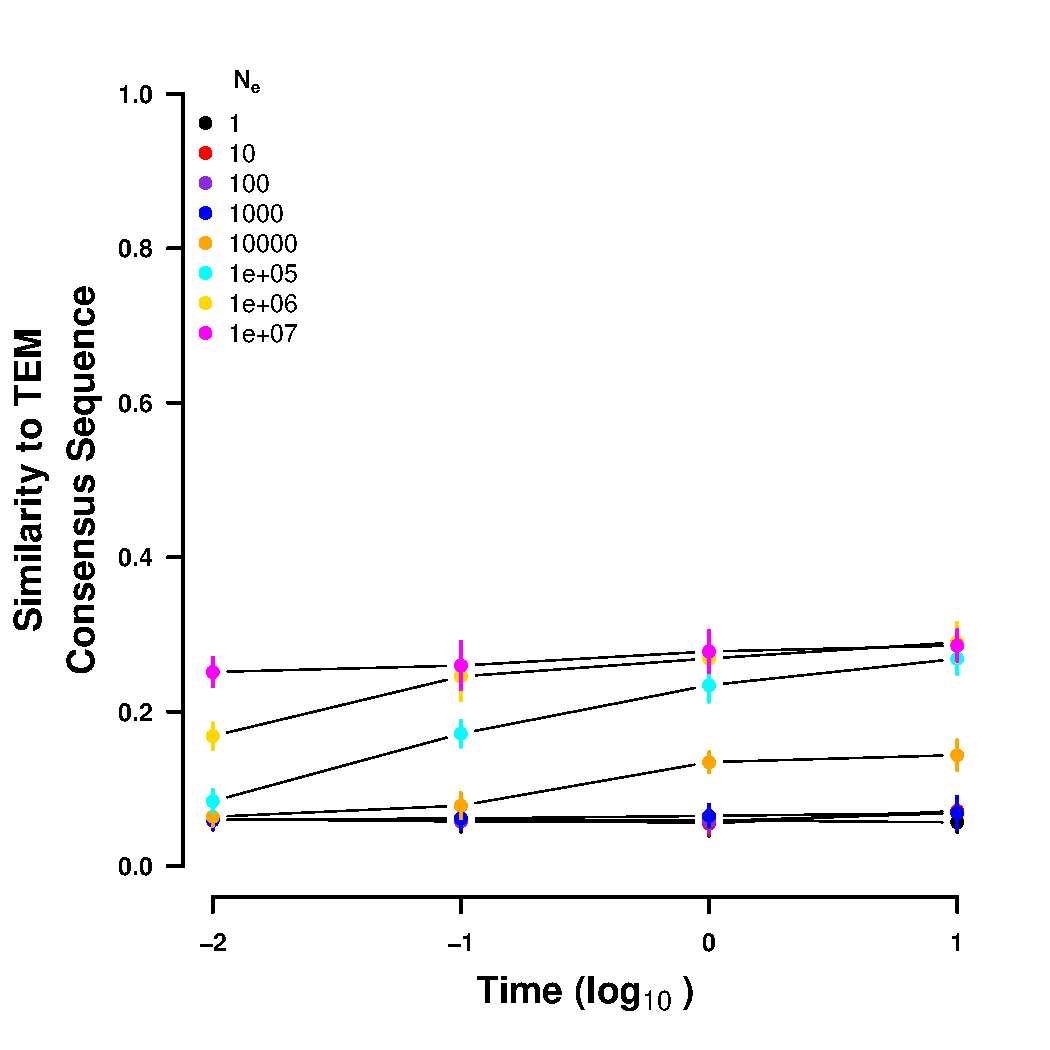
\includegraphics[width=.45\textwidth]{img/simulated_dist_time_SELAC_random.pdf}
    \end{subfigure}
    \begin{subfigure}
        \centering
        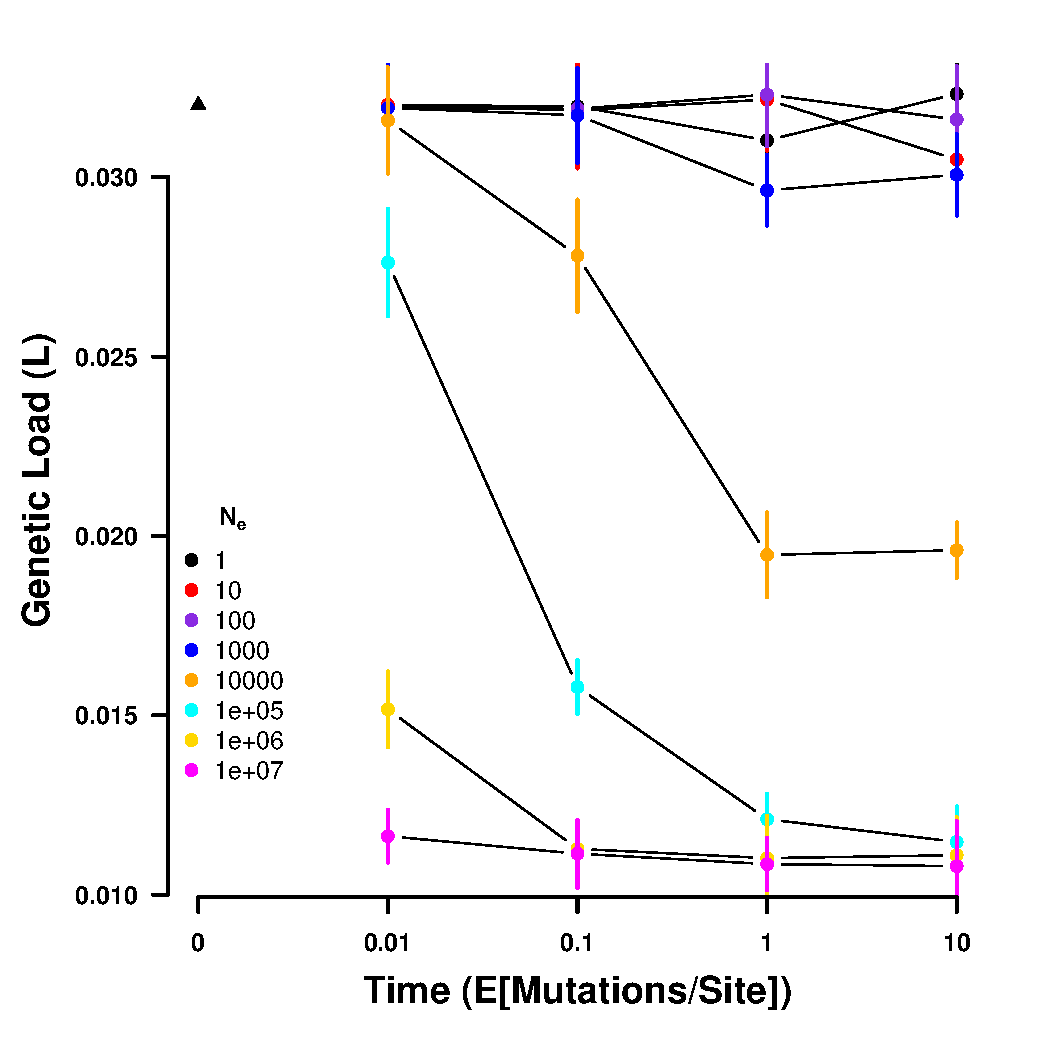
\includegraphics[width=.45\textwidth]{img/simulated_gl_time_SELAC_random.pdf}
    \end{subfigure}
    \caption{{Sequences simulated from a random codon sequence under the site specific selection on amino acids estimated using \selac. 
    (left) Sequence similarity to the observed consensus sequence at various times for a range on values of $N_e$.
    (right) Genetic load of the simulated sequences at various times for a range on values of $N_e$.
    Time is given in number of expected mutations.
    Points indicate sample means and vertical bars indicate standard deviations. Initial sequence is the inferred ancestral state of the TEM variants and not shown.}}
    \label{fig:selac_sim_rand}
\end{figure}

\begin{figure}[h]
    \centering
    \begin{subfigure}
        \centering
        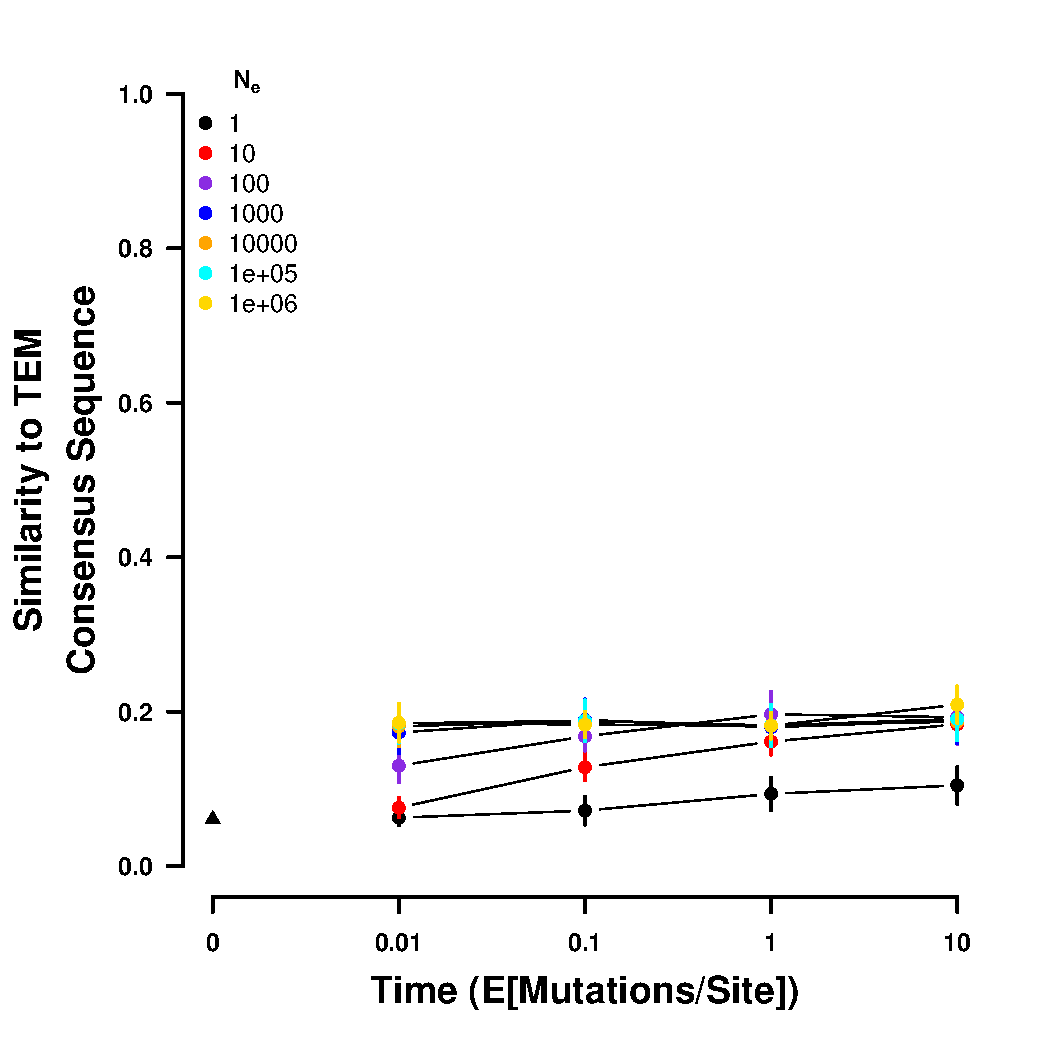
\includegraphics[width=.45\textwidth]{img/simulated_dist_time_DMS_random.pdf}
    \end{subfigure}
    \begin{subfigure}
        \centering
        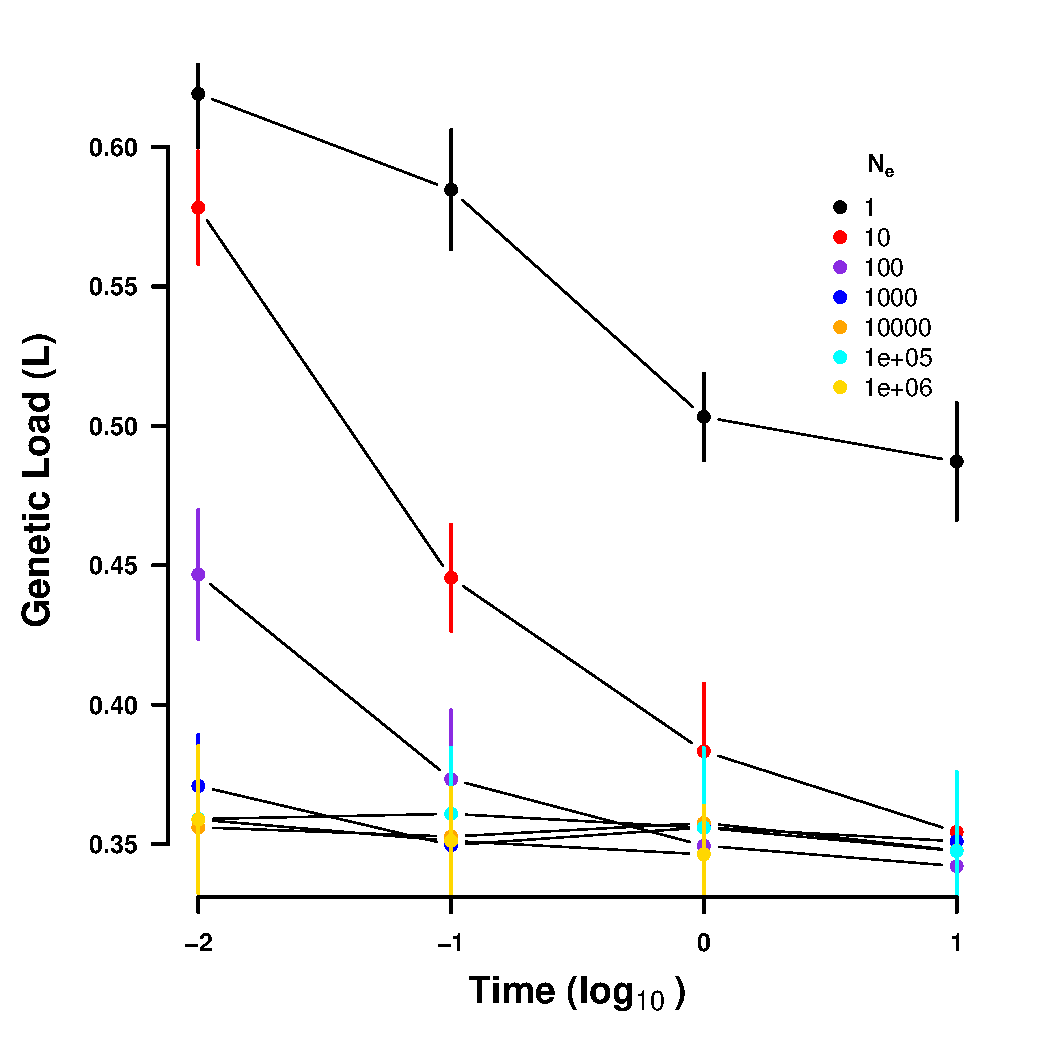
\includegraphics[width=.45\textwidth]{img/simulated_gl_time_DMS_random.pdf}
    \end{subfigure}
    \caption{{Sequences simulated from a random codon sequence under the site specific selection on amino acids estimated using deep mutation scanning. 
    (left) Sequence similarity to the observed consensus sequence at various times for a range on values of $N_e$.
    (right) Genetic load of the simulated sequences at various times for a range on values of $N_e$.
    Time is given in number of expected mutations.
    Points indicate sample means and vertical bars indicate standard deviations. Initial sequence is the inferred ancestral state of the TEM variants and not shown.}}
    \label{fig:selac_sim_rand}
\end{figure}

\begin{figure}[h]
    \centering
    \begin{subfigure}
        \centering
        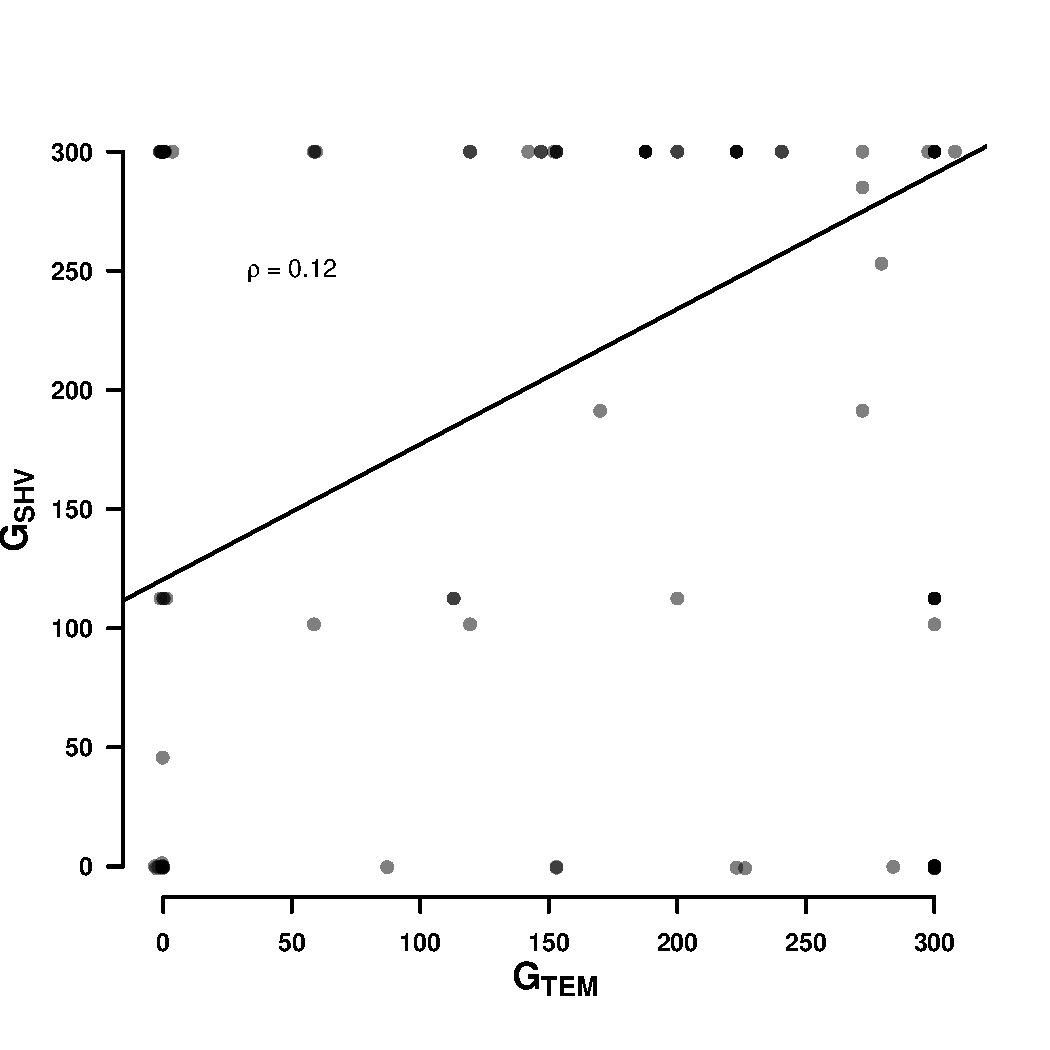
\includegraphics[width=.45\textwidth]{img/g_shift_lac.pdf}
    \end{subfigure}
    \begin{subfigure}
        \centering
        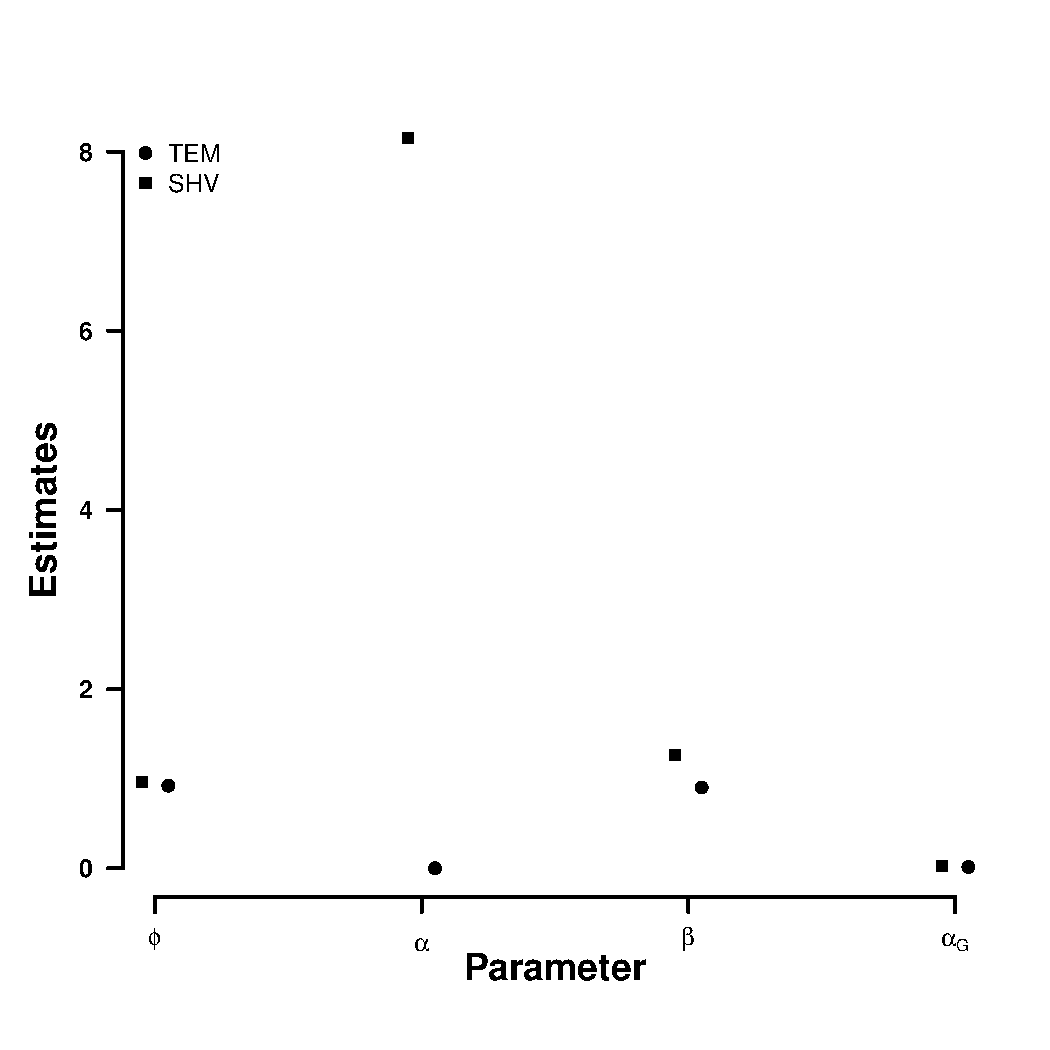
\includegraphics[width=.45\textwidth]{img/TEM_SHV_2016_par_comp.pdf}
    \end{subfigure}
    \caption{Comparisson of selection related parameters between TEM and SHV.}
    \label{fig:tem_shv_param_comp}
\end{figure}

\end{document}
